\subsection{Neural network design, training and classification}
\label{sec:des-class}
Two networks identify the text and writer of each line. Both extract stroke features with the same convolutional architecture, but their trained weights and output heads are separate. The text reader preserves horizontal order using a CNN and BiLSTM sequence model~\cite[pp.~4--5]{kizilirmak2023}. The writer head combines features across the line.

\subsubsection{Training data, labels and evaluation separation}
IAM lines~\cite{marti2002} and photographed samples provide transcripts and writer labels. The evaluated set contains six IAM writers (150, 152, 153, 384, 552 and 588) and five personal contributors. The personal pages were written on paper, photographed and paired with line transcripts. The eleven-writer set defines the reported classifier and stored style profiles.

The writer corpus contains 517 IAM and 669 personal lines. One IAM page per writer is held out, while a seeded 15\% split selects personal validation lines. This gives 1031 training and 155 validation lines. The final common evaluation contains 156 re-extracted lines, so it is reported separately from training validation. The text reader uses a joint corpus of Teklia pre-cut IAM and personal lines. Its complete historical training split is not retained.

Blank or unusable lines and printed prompts are excluded before pairing crops with labels. Augmentation stays within the training partition. Personal line holdout can share a page or capture session with training. The reader corpus and glyph-profile pages are also separate inputs, so a line held out from one model is not automatically excluded from all project data.

\subsubsection{Shared convolutional feature extractor}
The input is a batch of grey $64\times640$ line crops, shaped $(B,1,64,640)$ for batch size $B$. Intensity scaling to $[-1,1]$ makes dark ink positive and white padding negative. A learned kernel $W$ and bias $b$ calculate local responses from input $X$~\cite[pp.~6--8]{lecun1998}.
\begin{equation}
z_{o,y,x}=b_o+\sum_c\sum_{i,j}W_{o,c,i,j}X_{c,y+i,x+j}.
\label{eq:des-conv}
\end{equation}

The sums cover input channels and kernel positions. Input patches are rearranged into a matrix for multiplication by flattened kernels, avoiding a Python loop for every pixel operation~\cite{chellapilla2006}.

Batch normalisation uses channel mean $\mu_B$ and variance $\sigma_B^2$ during training, followed by learned scale $\gamma$ and offset $\beta$~\cite[pp.~4--5]{ioffe2015}.
\begin{equation}
\widehat z=\frac{z-\mu_B}{\sqrt{\sigma_B^2+\epsilon}},\qquad
y=\gamma\widehat z+\beta.
\label{eq:des-bn}
\end{equation}

The constant $\epsilon$ stabilises division. Inference uses stored running statistics. ReLU applies $\max(0,y)$, retaining positive responses with a simple nonlinear operation. Max pooling retains the strongest response in each local window. Table~\ref{tab:des-backbone} gives the resulting feature dimensions.
\begin{table}[!htbp]\centering\small
\begin{tabularx}{\linewidth}{|l|X|l|}
\hline\textbf{Stage}&\textbf{Operation}&\textbf{Output excluding batch}\\\hline
Input&Aspect-preserving line fit and intensity scaling&$1\times64\times640$\\\hline
1&Two $3\times3$ convolutions, each with batch normalisation and ReLU; $2\times2$ max pool&$32\times32\times320$\\\hline
2&Four convolution/normalisation/ReLU blocks; $2\times2$ max pool&$64\times16\times160$\\\hline
3&Six convolution/normalisation/ReLU blocks&$128\times16\times160$\\\hline
Height reduction&Maximum over the remaining height&$128\times1\times160$\\\hline
\end{tabularx}
\caption{Convolutional stages and feature dimensions.}
\label{tab:des-backbone}
\end{table}

Two spatial pools reduce the width to 160 columns. The final maximum over height leaves 128 features per column. Figure~\ref{fig:des-firstfeatures} shows the input Owen line and three strong feature channels before the first spatial pool. Their scales are independent, so darkness cannot be compared as an absolute value between channels. The complete layer sequence is retained in Figure~\ref{fig:vt-featurestack} in the appendix.
\begin{figure}[H]\centering
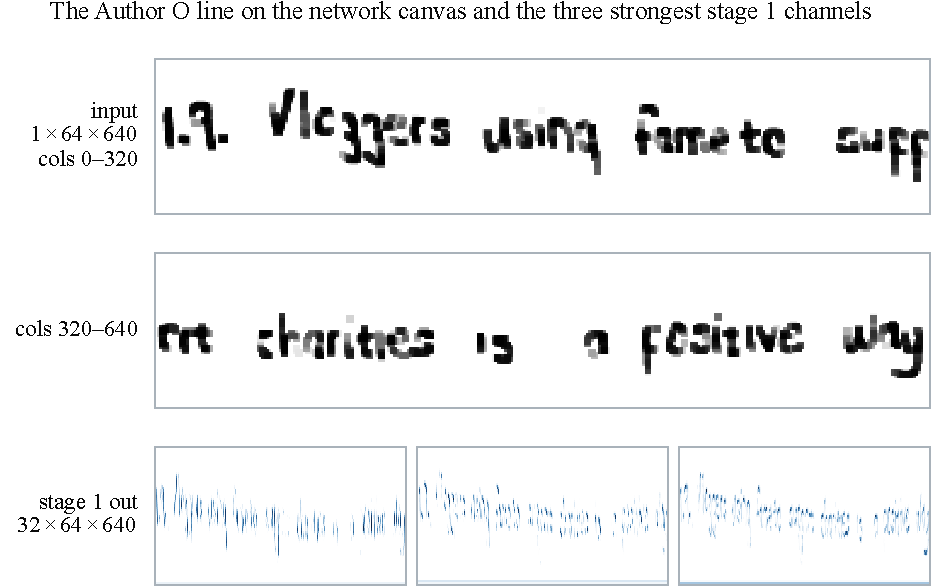
\includegraphics[width=\linewidth]{Figures/design-owen-first-features.pdf}
\caption{Input line and first convolutional features.}
\label{fig:des-firstfeatures}
\end{figure}

In the worked convolution, the weighted sum and bias give $z\simeq-1.15$. Batch normalisation gives $-8.54$, which ReLU sets to zero. The patch, learned values and full substitution are retained in Appendix~\ref{app:worked-design-calculations}.

\subsubsection{Text recognition using sequence modelling and CTC}
Figure~\ref{fig:des-network} shows the text-reader path. Two bidirectional LSTM layers, each with 256 hidden units per direction, process the 160 feature columns. The first receives 128 features per frame. The second receives 512 after both directions are concatenated. A linear layer produces scores for 74 characters and blank. The writer classifier does not use these recurrent layers.
\begin{figure}[H]\centering
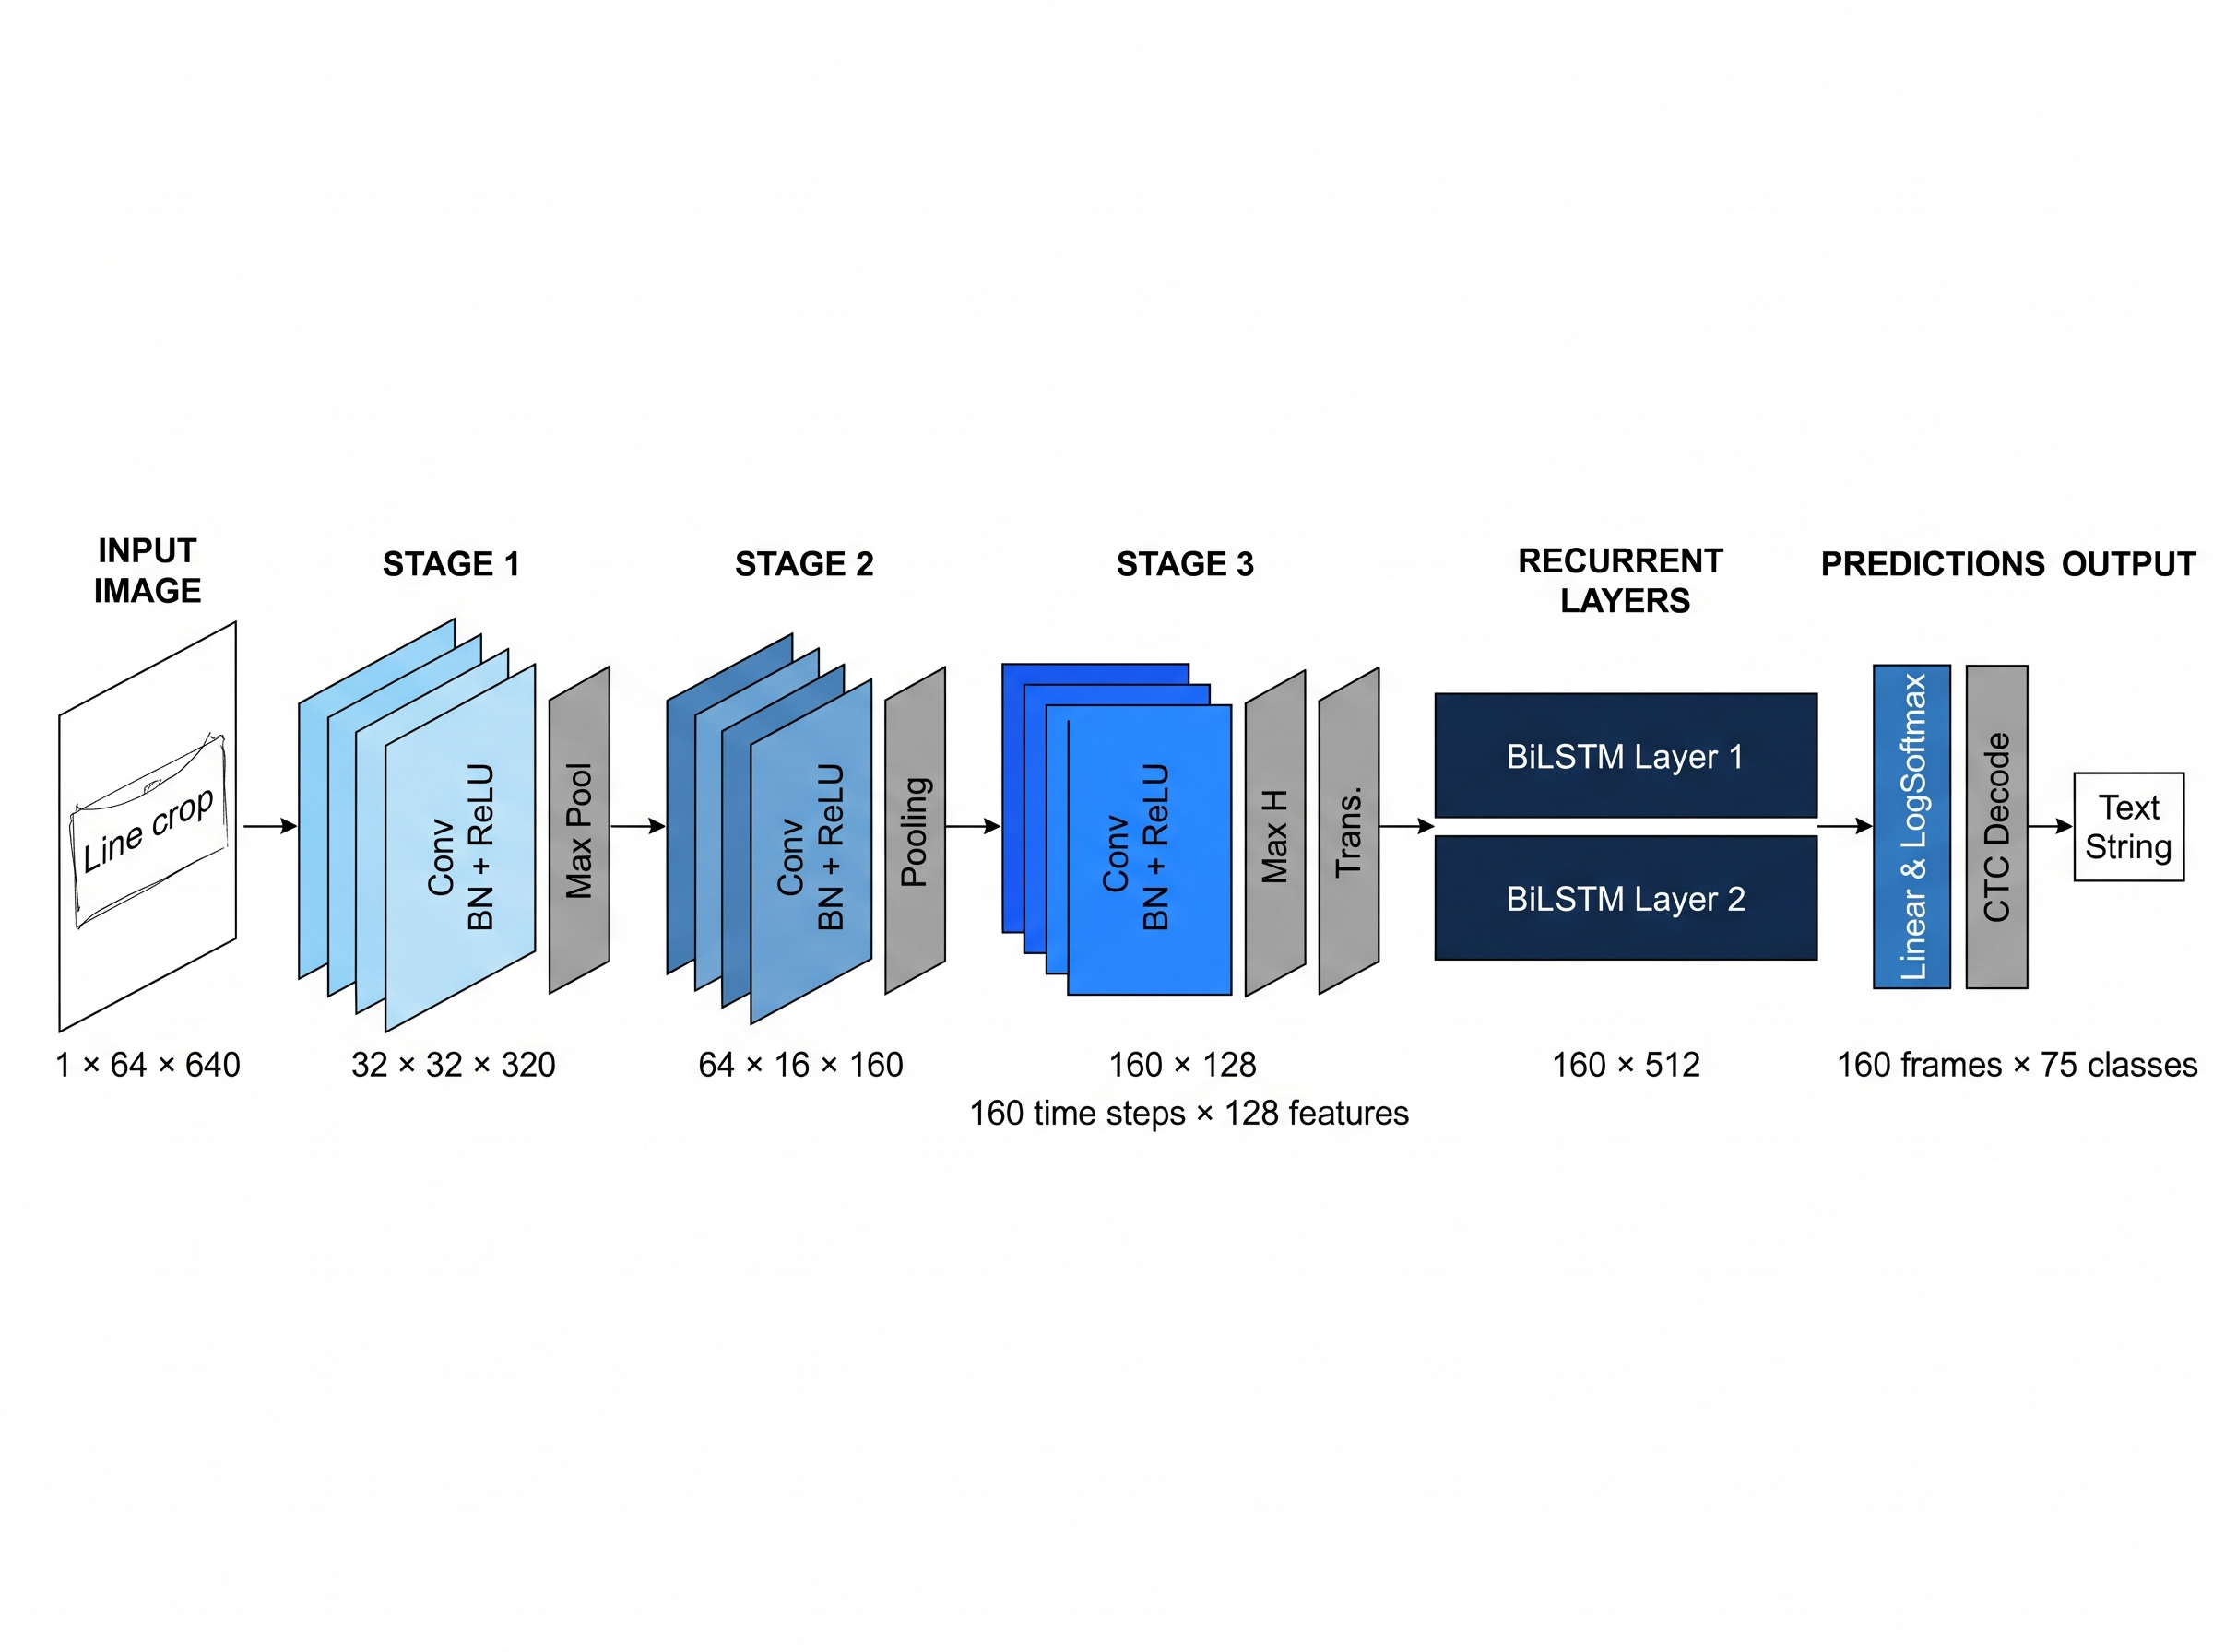
\includegraphics[width=0.96\linewidth,trim=0 130bp 0 134bp,clip]{Figures/BiLSTMCRNN.jpeg}
\caption{Text-reader architecture.}
\label{fig:des-network}
\end{figure}

The LSTM cell state $c_t$ carries memory between frames. Input, forget and output gates are $i_t,f_t,o_t$, with candidate update $g_t$ and hidden output $h_t$~\cite[p.~5]{graves2013}.
\begin{equation}
c_t=f_t\odot c_{t-1}+i_t\odot g_t,\qquad
h_t=o_t\odot\tanh(c_t).
\label{eq:des-lstm}
\end{equation}

The gates depend on the current feature vector and previous hidden state. Sigmoid $\sigma(a)=1/(1+e^{-a})$ bounds the gates between zero and one, while $\tanh$ bounds the candidate update. The reverse direction supplies context from the other end of the line. The implementation omits cell-to-gate peephole connections.

CTC trains from a line transcript without labelled character positions~\cite[pp.~2--3]{graves2006}. It sums frame paths $\pi$ whose collapse $\mathcal B$ produces transcript $\boldsymbol\ell$, using probabilities $p_t$ over $T=160$ frames.
\begin{equation}
\mathcal L_{\mathrm{CTC}}=-\log\sum_{\pi:\mathcal B(\pi)=\boldsymbol\ell}
\prod_{t=1}^{T}p_t(\pi_t).
\label{eq:des-ctc}
\end{equation}

Collapse merges consecutive repeats before removing blanks. Thus $a,a,\varnothing,b,b$ becomes ``ab'', while $a,\varnothing,a$ gives ``aa''. The dynamic programme uses blank-interleaved target states and log probabilities. For $L$ labels and $r$ adjacent repeated pairs, at least $L+r$ frames are required.

Greedy inference selects the most probable class at each frame and applies that collapse rule. No language model or lexicon is used. Figure~\ref{fig:vt-lattice} compares greedy decoding with alignment constrained to the known Owen transcript. This line is a worked example containing adjacent \texttt{g}s, which require separated emission runs. The greedy result matches its transcript and blank carries about 46\% of mean frame probability.
\begin{figure}[H]\centering
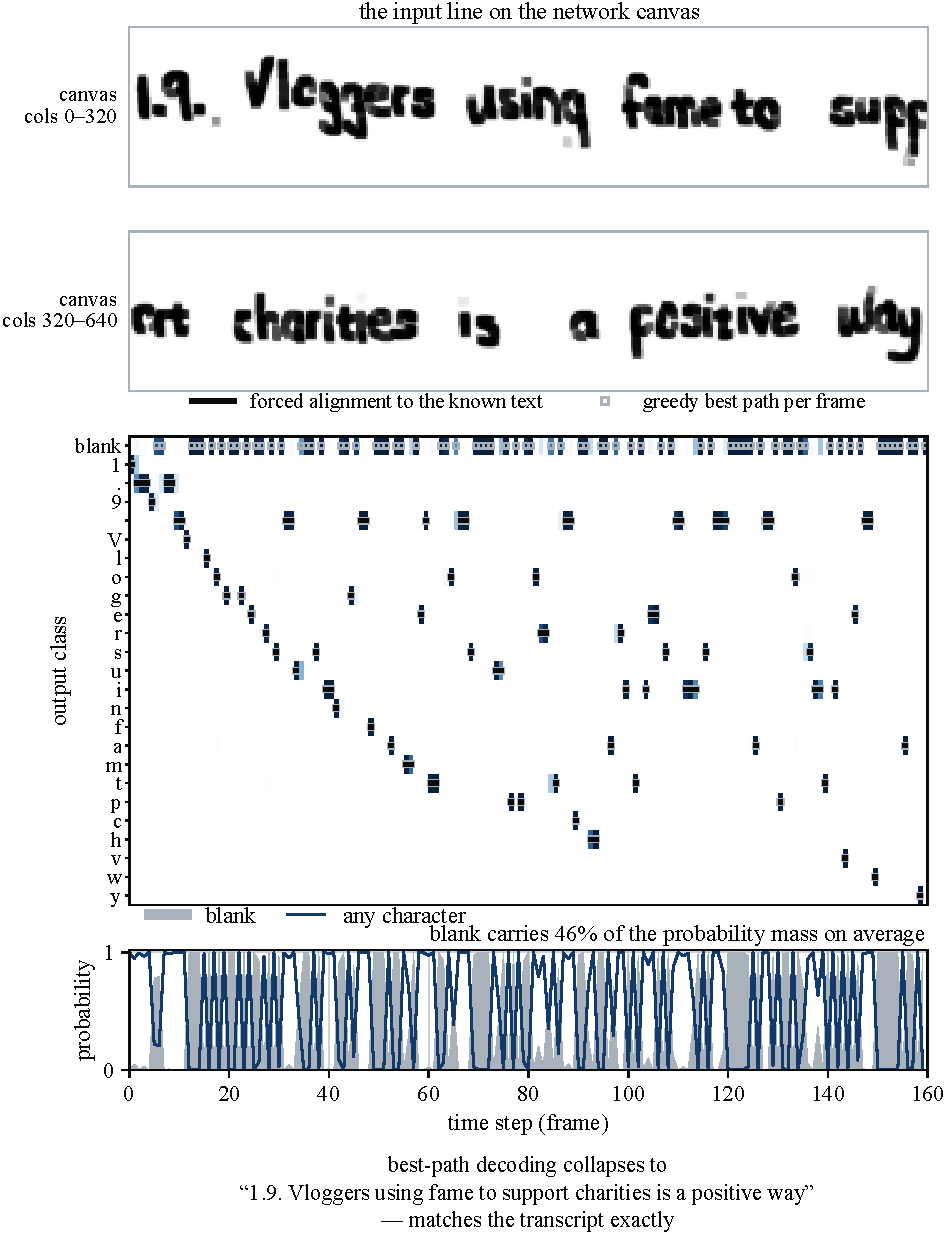
\includegraphics[width=\linewidth]{Figures/VisualTests/T36_ctc_lattice.pdf}
\caption{CTC decoding and forced alignment.}
\label{fig:vt-lattice}
\end{figure}

The numerical backward pass uses target-state occupancy $q_{t,k}$, total path probability $Z$ and logits $z_{t,k}$. Forward score $\alpha$ includes the current emission, while backward score $\beta$ includes only later emissions~\cite[pp.~4--6]{graves2006}.
\begin{equation}
q_{t,k}=\sum_{s:\ell'_s=k}\exp(\alpha_{t,s}+\beta_{t,s}-\log Z),
\qquad \frac{\partial\mathcal L}{\partial z_{t,k}}=p_t(k)-q_{t,k}.
\label{eq:des-ctcgrad}
\end{equation}

The batch average is applied without target-length division in the numerical trainer. Appendix~\ref{app:des-training-procedures} gives the full recurrence, and Appendix~\ref{app:worked-design-calculations} retains the recorded state and derivative calculations.

\subsubsection{Writer identification and stroke normalisation}
\label{sec:des-shapenamer}
The writer head averages the 160 feature columns into 128 values. A 96-unit hidden layer, ReLU and a $K$-class output identify the writer. Dropout probability 0.2 is active only during training~\cite[pp.~1931, 1934]{srivastava2014}.

The first classifier used the photographed ink directly. Ink width is a useful writer cue~\cite[p.~162]{brink2012}, but the gantry uses its own pen. The later classifier therefore uses normalised strokes so that original and reproduced writing are compared more through their geometry. Binarisation, Zhang--Suen thinning and square dilation form that input~\cite[p.~237]{zhang1984},~\cite[p.~533]{haralick1987}.
\begin{equation}
I_s=255\left[1-\delta_k\bigl(\operatorname{thin}(M)\bigr)\right],\quad
w=\operatorname{clip}\bigl(\operatorname{round}(\rho h_x),2,9\bigr),\quad
k=2\lfloor w/2\rfloor+1.
\label{eq:des-strokenorm}
\end{equation}

Here $h_x$ is estimated x-height, $\rho$ is the width fraction and $k$ is an odd dilation-kernel size. The selected fraction is 0.17. Figure~\ref{fig:des-strokenorm} shows Owen and Yeukita to illustrate different letter shapes under the same preparation. The original ink is reduced to a centreline before a controlled width is restored. Thresholding or thinning can still damage faint and touching strokes.
\begin{figure}[H]\centering
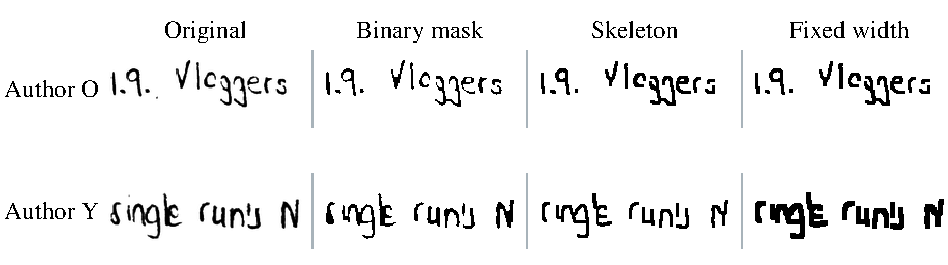
\includegraphics[width=\linewidth]{Figures/design-stroke-normalisation.pdf}
\caption{Stroke normalisation on two writers.}
\label{fig:des-strokenorm}
\end{figure}

The supplied sweep uses the same eleven writers and held-out partition, with a 50-epoch budget for each width. Table~\ref{tab:des-widthselection} gives the best saved epoch and validation score.
\begin{table}[!htbp]\centering\small
\begin{tabular}{|c|c|c|}
\hline\textbf{Width fraction $\rho$}&\textbf{Best saved epoch}&\textbf{Held-out writer accuracy}\\\hline
0.06&38&98.06\%\\\hline
0.09&43&97.42\%\\\hline
0.11&39&98.06\%\\\hline
0.17&43&99.35\%\\\hline
\end{tabular}
\caption{Stroke-width selection using the same eleven-writer population and held-out partition.}
\label{tab:des-widthselection}
\end{table}

The best observed width was 0.17. Preparation and inference use that stored setting rather than the 0.14 module default. Odd integer kernels mean that nearby fractions can give the same image on one crop, as shown in Appendix~\ref{app:vt-width}. The sweep selects preprocessing and is kept separate from final qualification.

\subsubsection{Training procedure and model selection}
\label{sec:des-training}
The backbone and task head are updated together. Training uses variance-scaled convolution weights and initial normalisation scales of one with zero offsets. Shear, small rotations, perspective changes and elastic distortion vary the training images while preserving labels. Validation uses a fixed preparation path without augmentation or dropout.

The reader minimises CTC loss. The writer minimises cross-entropy $-\log p_y$ for true writer $y$, with logit derivative $p_k-\mathbf1[k=y]$~\cite[p.~6]{graves2013}. Table~\ref{tab:des-training} records implemented numerical defaults, rather than settings recovered for every historical run.
\begin{table}[!htbp]\centering\small
\begin{tabularx}{\linewidth}{|l|X|X|}
\hline\textbf{Setting}&\textbf{Reader}&\textbf{Writer classifier}\\\hline
Objective&CTC loss&Cross-entropy\\\hline
Optimiser&RMSprop&AdamW\\\hline
Initial learning rate&$10^{-3}$ default&$10^{-3}$ default\\\hline
Weight decay&$10^{-5}$&$10^{-4}$\\\hline
Learning-rate schedule&Plateau reduction, factor 0.5, patience 5, minimum $10^{-5}$&Cosine annealing over the configured run\\\hline
Gradient-norm clipping&Not applied by the current NumPy text loop&Maximum norm 5\\\hline
Best-checkpoint criterion&Lowest validation loss&Highest validation accuracy\\\hline
\end{tabularx}
\caption{Training settings implemented in the first-principles trainer. The table describes implemented defaults rather than a recovered record of every completed training run.}
\label{tab:des-training}
\end{table}

Joint reader training supports controlled personal-sample representation, with default fraction 0.20. Reader checkpoints are selected by validation loss and writer checkpoints by validation accuracy. Forward caches retain the quantities needed for differentiation. Algorithm~\ref{alg:des-train} in Appendix~\ref{app:des-training-procedures} gives the update procedure. The supplied first-principles training records are retained in Appendix~\ref{app:training-records}.

\subsubsection{First principles and framework implementations}
\label{sec:des-implementations}
The numerical route implements forward operations, backward operations, losses and optimiser updates using NumPy array arithmetic. The framework route expresses the corresponding architecture through PyTorch layers and automatic differentiation. Both use the project's preparation and named-array format, which the numerical inference path reads.

Table~\ref{tab:dis-training} compares trained models on common original validation material. The reader scores differ by 0.33 percentage points and writer scores by 2.57 points. These comparisons support the first-principles implementation without treating separately trained models as identical. Training logs and checkpoint identities are retained in the appendix.
\begin{table}[!htbp]\centering\small
\begin{tabularx}{\linewidth}{Xrr}\toprule
\textbf{Common validation material}&\textbf{Library route / \%}&\textbf{First principles / \%}\\\midrule
Reader, public IAM lines&94.12&94.39\\
Reader, photographed lines&93.33&94.42\\
Reader, pooled character accuracy&94.06&94.39\\
Writer, 156 original lines&98.08&95.51\\\bottomrule
\end{tabularx}
\caption{Training-route comparison on common data.}
\label{tab:dis-training}
\end{table}

The two CTC training reductions also differ. The numerical route averages sequence losses across the batch. The framework default divides by target length before averaging and zeroes impossible-alignment losses~\cite{pytorchctc}. Controlled training comparisons must match these choices. Table~\ref{tab:des-implementations} records the operations and data interfaces.

\subsubsection{Network verification and design limitations}
\label{sec:des-netverify}
A numerical comparison uses identical inputs, parameters and precision, with random masks matched or disabled. A learning comparison instead evaluates trained predictions. Table~\ref{tab:des-numericalcheck} gives the archived float64 check on two random images, including the reader and an earlier thirteen-output writer head.
\begin{table}[H]\centering\small
\begin{tabularx}{\linewidth}{|X|r|r|}
\hline\textbf{Recorded comparison metric}&\textbf{Reader}&\textbf{Writer classifier}\\\hline
Maximum logit difference / maximum magnitude&$2.12\times10^{-14}$&$3.04\times10^{-15}$\\\hline
Absolute loss difference&$1.14\times10^{-13}$&$1.78\times10^{-15}$\\\hline
Worst ranked gradient relative $L_2$ difference&$2.80\times10^{-13}$&$6.01\times10^{-14}$\\\hline
\end{tabularx}
\caption{Archived float64 operation comparison.}
\label{tab:des-numericalcheck}
\end{table}

The logit metric uses the maximum absolute difference divided by the larger maximum magnitude, with a $10^{-8}$ floor. Gradient comparisons use relative $L_2$ difference and exclude near-zero tensors from the worst-ranked summary. The check supports the tested operations, rather than every possible training run.

The archive also contains a 500-line, 15-epoch learning comparison and an exhaustive 1024-path CTC check. The latter gives loss discrepancy $4.44\times10^{-16}$ and maximum derivative discrepancy $3.63\times10^{-11}$. Their fixtures and gradient checks are retained in Appendices~\ref{app:des-visual-tests} and~\ref{app:vt-gradient}.

Long-line resizing reduces fine detail, personal line splits share capture conditions, and the closed writer head always selects among its trained identities. These limits guide the examples and held-out evaluation. Final recognition and writer results are reported in Section~\ref{sec:results}.
\FloatBarrier
